\section{Handling merge conflicts}
\begin{frame}[fragile]
  \slidetitle
  This section covers the following topics:
  \begin{itemize}
    \pause
    \item Solve merge conflicts
    \pause
    \item Using diff tools
    \pause
    \item 3 way merge
  \end{itemize}
\end{frame}

\subsection{A requirement change}
\begin{frame}[fragile]
    \subslidetitle
  Our customer changed his mind about the color of the green moon.
  \newline \vspace{1em}
  \#4 Change the color of the green moon to red.

  Implement the change in moon.js following this diff:
\begin{lstlisting}
(*\textcolor[HTML]{18B2B2}{@@ -4,7 +4,7 @@}*) var moons = [];
 init();
 moon( "blue" );
 moon( "white" );
(*\textcolor{red}{-}*)(*\textcolor{red}{moon( "green" );}*)
(*\textcolor[HTML]{00AA00}{+}*)(*\textcolor[HTML]{00AA00}{moon( "red" );}*)
 animate();
\end{lstlisting}

\end{frame}

\subsection{Display differences}
\begin{frame}[fragile]
    \subslidetitle
  The \cmd{git difftool} will run the application of your choice to display differences:
  \begin{lstlisting}
(*\textcolor[HTML]{18B2B2}{(master)}*) $ (*\textcolor[HTML]{0000AA}{git difftool --tool kdiff3}*)
Viewing (1/1): 'moon.js'
Launch 'kdiff3' [Y/n]: Y
\end{lstlisting}

  \vspace{1em}
  \centerline{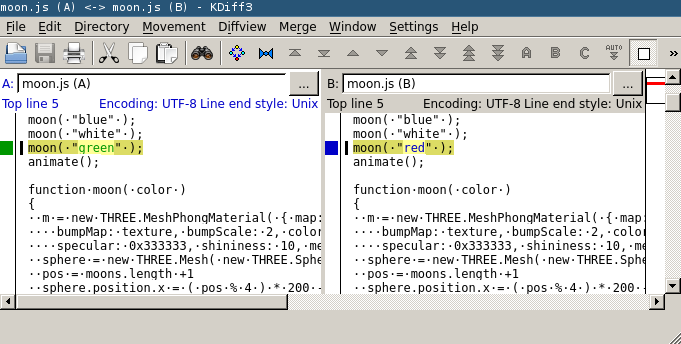
\includegraphics[width=8cm]{../screen/git-difftool-kdiff3.png}}

  Note: This can be helpful to call an external diff toll like kdiff3 or meld, especially to have a side-by-side diff.

\end{frame}


\subsection{Update feature-flag-color}
\begin{frame}[fragile]
    \subslidetitle
  Commit your changes on master:
\begin{lstlisting}
(*\textcolor[HTML]{18B2B2}{(master)}*) $ (*\textcolor[HTML]{0000AA}{git commit -a -m "change the green moon color to red, implements \#4"}*)
(*\textcolor[HTML]{18B2B2}{(master)}*) $ (*\textcolor[HTML]{0000AA}{git checkout feature-color-flag}*)
\end{lstlisting}

  Add a comment to the green moon like defined in the following diff:
  \begin{lstlisting}
(*\textcolor[HTML]{18B2B2}{@@ -4,7 +4,7 @@}*) var moons = [];
 init();
 moon( "blue" );
 moon( "white" );
(*\textcolor{red}{-}*)(*\textcolor{red}{moon( "green" );}*)
(*\textcolor[HTML]{00AA00}{+}*)(*\textcolor[HTML]{00AA00}{moon( "green" ); // no requirement}*)
 animate();
\end{lstlisting}

  Commit your changes:
  \begin{lstlisting}
(*\textcolor[HTML]{18B2B2}{(master)}*) $ (*\textcolor[HTML]{0000AA}{git commit -a -m "add comment about requirement for the green color"}*)
\end{lstlisting}
\end{frame}

\subsection{Merge feature-flag-color}
\begin{frame}[fragile]
    \subslidetitle

  The feature-flag-color is ready to be merged to master, try to merge the feature-flag-color branch to master:
  \begin{lstlisting}
(*\textcolor[HTML]{18B2B2}{(feature-flag-color)}*) $ (*\textcolor[HTML]{0000AA}{git checkout master}*)
Switched to branch 'master'
Your branch is up-to-date with 'origin/master'.
(*\textcolor[HTML]{18B2B2}{(master)}*) $ (*\textcolor[HTML]{0000AA}{git merge feature-flag-color}*)
Auto-merging moon.js
CONFLICT (content): Merge conflict in moon.js
Automatic merge failed; fix conflicts and then commit the result.
\end{lstlisting}

Here we go, our first conflict, keep calm, do not panic, we use \cmd{git}
\end{frame}

\subsection{Display the conflict}
\begin{frame}[fragile]
    \subslidetitle

  First we want to display the conflicting file with \cmd{git difftool}:
  \begin{lstlisting}
(*\textcolor[HTML]{18B2B2}{(master|MERGING)}*) $ (*\textcolor[HTML]{0000AA}{git difftool}*)
diff --cc moon.js
index 72886cb,861507e..0000000
--- a/moon.js
+++ b/moon.js
(*\textcolor[HTML]{18B2B2}{@@@ -4,7 -4,7 +4,11 @@@}*) var moons = []
  init();
  moon( "blue" );
  moon( "white" );
(*\textcolor[HTML]{00AA00}{++}*)(*\textcolor[HTML]{00AA00}{<<<<<<< HEAD}*)
(*\textcolor[HTML]{00AA00}{+}*) (*\textcolor[HTML]{00AA00}{moon( "red" );}*)
(*\textcolor[HTML]{00AA00}{++}*)(*\textcolor[HTML]{00AA00}{=======}*)
(*\textcolor[HTML]{00AA00}{+}*) (*\textcolor[HTML]{00AA00}{moon( "green" ); // no requirement}*)
(*\textcolor[HTML]{00AA00}{++}*)(*\textcolor[HTML]{00AA00}{>>>>>>> feature-flag-color}*)
  animate();

  function moon( color )
\end{lstlisting}
\end{frame}

\subsection{Resolve a conflict}
\begin{frame}[fragile]
    \subslidetitle
  Use \cmd{git mergetool} and select an external merge tool like kdiff3, vimdiff to resolve a conflict:

  \begin{lstlisting}
(*\textcolor[HTML]{18B2B2}{(master|MERGING)}*) $ (*\textcolor[HTML]{0000AA}{git mergetool}*)
Merging:
moon.js

Normal merge conflict for 'moon.js':
  {local}: modified file
  {remote}: modified file
\end{lstlisting}

  Note: the \cmd{kdiff3} automatically starts since we configured it in the \cmd{\textasciitilde/.gitconfig} file
  \begin{lstlisting}
...
[merge]
  tool = kdiff3
...
\end{lstlisting}
\end{frame}

\subsection{Three way merge}
\begin{frame}[fragile]
    \subslidetitle
  Have a look at the \cmd{kdiff3} application, right click on the \textcolor{red}{?<Merge Conflict>} and select the apporpriate resolution:
  \newline \vspace{1em}
  \centerline{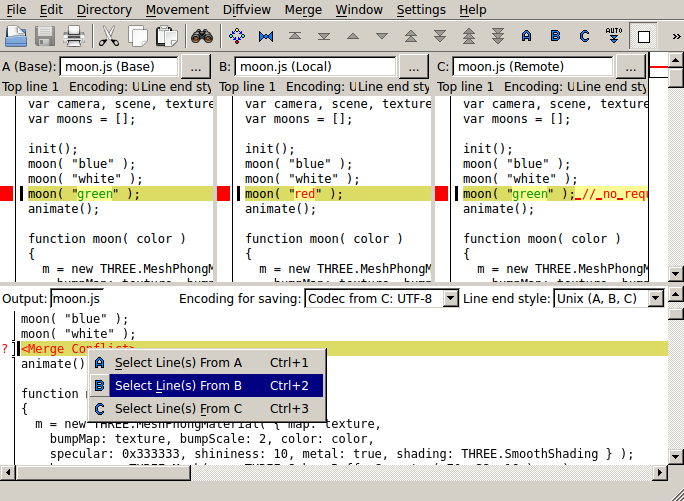
\includegraphics[width=8cm]{../screen/git-mergetool-kdiff3-resolve.png}}

\end{frame}

\subsection{Finish merge}
\begin{frame}[fragile]
    \subslidetitle
  The \cmd{git status} gives some hints how to finialize the merge conflict resolution:
  \begin{lstlisting}
(*\textcolor[HTML]{18B2B2}{(master|MERGING)}*) $ (*\textcolor[HTML]{0000AA}{git status}*)
On branch master
Your branch is ahead of 'origin/master' by 1 commit.
  (use "git push" to publish your local commits)
All conflicts fixed but you are still merging.
  (use "git commit" to conclude merge)
...
\end{lstlisting}

  Just use \cmd{git commit} to finish the merge, this will automatically open the text editor, save and quit:
  \begin{lstlisting}
(*\textcolor[HTML]{18B2B2}{(master|MERGING)}*) $ (*\textcolor[HTML]{0000AA}{git commit}*)
Merge branch 'feature-flag-color' into master
# Conflicts:
#       moon.js
\end{lstlisting}
  You successfully resolved you first conflict with git, not so difficult !?

\end{frame}

